\section{Geheugenbeheer}

Effectief geheugenbeheer is essentieel bij een systeem met multiprogrammering. Geheugen moet efficiënt worden toegewezen om zoveel mogelijk processen in het geheugen te laden zodat de processortijd optimaal benut wordt.

\subsection{Vereisten voor geheugenbeheer}

Het geheugenbeheer vereist de volgende voorwaarden:

\begin{multicols}{2}
\begin{itemize}
\item Relocatie
\item Bescherming
\item Delen
\item Logische indeling
\item Fysieke indeling
\end{itemize}
\end{multicols}

\subsubsection{Relocatie}

De programmeur weet meestal niet waar het programma in het geheugen geplaatst zal worden bij uitvoering. Tijdens uitvoering van het programma kan het terug naar schijf geswapt worden om dan terug naar het geheugen geplaatst te worden op een andere locatie.

Geheugen verwijzingen moeten vertaald worden naar het echte fysieke geheugen adres. Een frame is een blok hoofdgeheugen met een vaste lengte.

Een pagina is een blok secundair geheugen met een vaste lengte.

Een segment is een blok geheugen in het secundair geheugen met een variabele lengte. Volgend procesbeeld toont de technische aandachtspunten voor adressering.



\begin{figure}[htp]
    \centering
            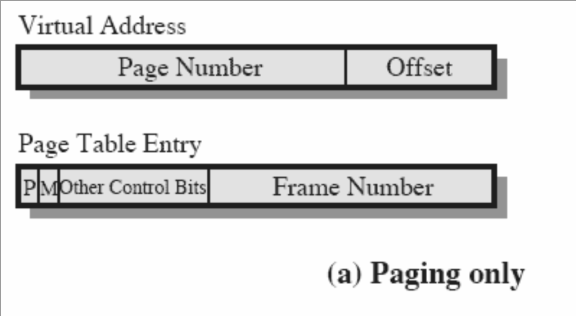
\includegraphics[width=4in]{img/pagineren.png}
        \caption{Paging only}
    \label{fig:Paging only}
\end{figure}


\subsubsection{Bescherming}

Processen moeten beschermd worden tegen verstoringen door andere processen:

\begin{itemize}
\item Processen mogen niet zonder toestemming naar geheugenlocaties in andere processen verwijzen.
\item Bij relocatie is de locatie van een programma in het hoofdgeheugen onbekend, dus is het onmogelijk absolute geheugenadressen te controleren bij het compilen.
\item Geheugenverwijzingen moeten dus at run time gecontroleerd worden.
\item De vereisten voor geheugenbescherming moeten voldaan zijn door de processor (hardware) in plaats van door het besturingssysteem (software).
\item Het BS kan niet anticiperen op alle geheugenverwijzingen die een programma kan gebruiken.
\end{itemize}


\subsubsection{Delen}

Bescherming van de processen is noodzakelijk maar het moet wel mogelijk zijn dat processen bepaalde delen van het geheugen delen. Het is ook beter om elk proces toegang te geven tot hetzelfde exemplaar van het programma, in plaats van dat elk proces zijn eigen kopie gebruikt. Dit is het overmatig gebruiken van het werkgeheugen.

\subsubsection{Logische indeling}

De meeste programma’s zijn ingedeeld in modules, waarvan sommige niet kunnen worden gewijzigd (alleen lezen, … ) en waarvan andere modules gegevens bevatten die wel mogen worden gewijzigd.

Voordelen van modules:


\begin{itemize}
\item Modules kunnen onafhankelijk worden geschreven en gecompileerd. Waarbij alle verwijzingen van de ene naar de andere module tijdens de uitvoering worden ingevuld door het systeem.
\item Verschillende modules kunnen andere beschermingsniveaus krijgen ten koste van wat overhead.
\item Het wordt mogelijk mechanismen te maken waarbij processen modules kunnen delen.
\end{itemize}


\subsubsection{Fysieke indeling}

Het is niet de programmeur zijn verantwoordelijkheid om het geheugen te beheren.

Het geheugen dat beschikbaar is voor een programma en zijn data kan niet genoeg zijn. Overlaying laat toe dat meerder modules kunnen worden toegekend aan hetzelfde geheugengebied, het is aan het hoofdprogramma om te zorgen dat de modules gewisseld worden.
